% Metódy inžinierskej práce

\documentclass[10pt,oneside,slovak,a4paper]{article}

\usepackage[slovak]{babel}
\usepackage{float}
%\usepackage[T1]{fontenc}
\usepackage[IL2]{fontenc} % lepšia sadzba písmena Ľ než v T1
\usepackage[utf8]{inputenc}
\usepackage{graphicx}
\usepackage{url} % príkaz \url na formátovanie URL
\usepackage{hyperref} % odkazy v texte budú aktívne (pri niektorých triedach dokumentov spôsobuje posun textu)

\usepackage{cite}
%\usepackage{times}

\pagestyle{headings}

\title{Využitie gamifikácie vo výučbe cudzích jazykov\thanks{Semestrálny projekt v predmete Metódy inžinierskej práce, ak. rok 2020/21, vedenie: Ing. Jozef Sitarčík}} % meno a priezvisko vyučujúceho na cvičeniach

\author{Peter Janoš\\[2pt]
	{\small Slovenská technická univerzita v Bratislave}\\
	{\small Fakulta informatiky a informačných technológií}\\
	{\small \texttt{xjanosp@stuba.sk}}
	}

\date{\small 20.10.2020} % upravte



\begin{document}

\maketitle

\begin{abstract}
Ovládanie cudzieho jazyka sa v dnešnej dobe považuje za nevyhnutné. Mnoho ľudí sa s cudzím jazykom, ako napríklad angličtina, stretáva už v ranom veku v školách a potom s ňou prichádzajú do kontaktu takmer každý deň na internete, v hudbe, vo filmoch alebo v článkoch, čo im pomáha sa ďalej rozvíjať. Existuje ale aj skupina ľudí, ktorí takéto možnosti nemali a chcú sa cudzí jazyk naučiť sami. No učenie sa cudzieho jazyka je zložitý proces a preto vznikli nové spôsoby vzdelávania, ktoré ho má zjednodušiť. Jeden z týchto nových spôsobov je takzvaná gamifikácia. Gamifikácia je relatívne nový koncept, ktorý spája zábavu s učením. Využíva herné elementy a dizajn, čo v teórii spríjemňuje atmosféru pri učení a taktiež odmieňa učiaceho sa za jeho pokroky, čo ho motivuje sa naďalej zlepšovať. Výsledky štúdií, ktoré sa venovali efektivite tejto stratégie ale preukázali zmiešané výsledky. V tomto článku sa budeme bližšie venovať gamifikácií ako takej, učeniu sa cudzieho jazyka a aj tomu ako môže táto stratégia pomáhať motivovať účastníka zapájať sa do tohto vzdelávacieho procesu.
\end{abstract}

\section{Úvod} \label{uvod}
Počítačové a mobilné hry sa stali súčasťou života mnohých ľudí. Aj preto môžeme čoraz častejšie vidieť, že sa nejakú formu hier snažia učitelia implementovať aj do vzdelávania. Takýmto spôsobom učenia sa je aj stále viac a viac populárnejšia gamifikácia, ktorej sa budeme venovať v tomto článku. Gamifikácia, by mohla byť novou metódou, ktorá by umožňovala učiteľom viac motivovať svojich študentov, aby sa efektívnejšie a rýchlejšie naučili druhý jazyk. 

Keďže je gamifikácia stále relatívne novým konceptom, nebolo na ňu vykonaných veľa štúdií, ktoré by potvrdzovali alebo vyvrátili jej efektívnosť. Štúdie, ktoré boli vykonané poukazovali na pozitívne výsledky pri vplyve na motiváciu učiaceho sa, no niektoré zase poukazovali na presný opak. Gamifikácia zatiaľ našla svoje využitie hlavne v marketingových alebo obchodných oblastiach.
~\cite{garland2015gamification}

Na začiatku článku sa budeme venovať niektorým dôležitým pojmom, ktoré sú potrebné na porozumenie celej problemaitky. Definujeme si pojem gamifikácia \ref{gamifikacia} a bližšie sa pozrieme aj na to, prečo je motivácia dôležitá pri učení.\ref{motivacia} V ďalšej časti sa budeme venovať spomínaným štúdiám vykonaných o gamifikácií\ref{studies}, ale aj na jej prvky, využitie, históriu a stále narastajúcu popularitu.\ref{gamificationsection} V predposlednej kapitole sa pozrieme na vplyv gamifikácie na výučbu cudzích jazykov. \ref{use}




\section{Dôležité definicie} \label{definicie}
\subsection{Definícia gamifikácue} \label{gamifikacia}
V tejto časti sa budeme venovať gamifikácií ako takej. Čo je to vlastne gamifikácia? Aj keď sa na prvý pohľad môže zdať, že gamifikácia a hra je to isté, nie je tomu tak. Hry ako počítačové alebo stolné hry hráme pre zábavu. Gamifikácie je však metóda, ktorú môžme použiť pre zlepšenie používateľského zážitku pri práci, alebo učení sa. Využíva herné prvky a herný dizajn v nehernom kontexte \ref{elements}, teda napríklad za iným účelom ako je samotné hranie hry. Ako napríklad získavanie bodov pri úspešnom riešení problému, odomykane nových úrovní alebo aj odmenenie virtuálnym odznakom. Princíp gamifikácie môžeme vidieť v aplikáciách ako napríklad:


\begin{itemize}
    \item Duolingo - Aplikácia na učenie cudzích jazykov, ktorá používateľa odmieňa za pokroky. Núti používateľa neustále opakovať nové učivo.
    \item Waze - Navigačná aplikácia, ktorá využíva gamifikáciu na získavanie informácií, čím zlepšuje svoju presnosť.
    \item Adidas - Internetový obchod, ktorý využíva gamifikáciu pri odmieňaní používateľa bodmi pri každom nákupe. Čím viac bodov má, tým má väčšie benefity.
\end{itemize}
\begin{center}
    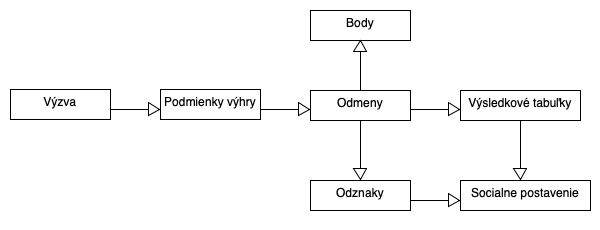
\includegraphics[scale = 0.5]{diagram.png}

\end{center}


\subsection{Motivácia a učenie} \label{motivacia}
Motivácia hrá pri učení sa veľmi dôležitú rolu. Byť motivovaný znaméná byť odhodlaný začať na niečom pracovať a aj to dokončiť. Človeka, ktorý necíti chuť ani inšpiráciu pracovať na niečom môžeme nazvať nemotivovaným. Na druhej strane, človeka, ktorý je podnietený a pripravený dotiahnuť svoju prácu do konca, môžeme nazvať motivovaným. Motivácia sa u ľudí nelíši len úrovňou (ako veľmi sú motivovaní), ale aj typom motivácie. Typy motivácie rozoznávame podľa postojov a cieľov, ktoré vedú človeka k tomu, aby konal. Tieto typy rozdeľujeme na vnútornú a vonkajšiu motiváciu. ~\cite{ryan2000intrinsic}

\subsubsection{Vnútorná motivácia} \label{vnutorna}
Vnútorná motivácia je definovaná ako vykonávanie činnosti skôr pre uspokojenie a zábavu, ktorú daná činnosť človeku prináša, ako pre nejakú odmenu alebo ako dôsledok nátlaku. Dobrým príkladom vnútornej motivácie je napríklad študent, ktorý je veľmi motivovaný učiť sa a pracovať na sebe, len kvôli tomu, že chce získať nové vedomosti a zručnosti a nie len kvôli tomu, aby dostal dobrú známku. ~\cite{ryan2000intrinsic}

\subsubsection{Vonkajšia motivácia} \label{vonkajsia}
Externá motivácia je presný opak. Je to vykonávanie nejakej činnosti len pre dosiahnutie nejakého výsledku. Ako napríklad odmena alebo vyhnutie sa nejakému trestu. Ako príklad môžme použiť študenta, ktorý na sebe pracuje len kvôli strachu z môžného trestu od rodičov, alebo študenta, ktorý študuje len preto, aby mal čo najlepšie známky.~\cite{ryan2000intrinsic}
Lepper (1988) tvrdí, že vnútorná motivácia poukazuje na lepšie výsledky. Výsledkom vonkajšej motivácie je nižšia celková úroveň motivácie a spomalenie procesu učenia sa po uplynutí nejakého času a to aj v gamifikovanom kontexte. To však neznamená, že vonkajšia motivácia nemôže byť používaná vo výučbe. Prvky vonkajšej motivácie môžu byť implementované do aktivít a môžu byť použité spôsobom, ktorý posilňuje vnútornú motiváciu študentov. Motivácia je nesmierne dôležitým faktorom pri študovaní cudzích jazykov. Je však veľmi náročné vyvolať a posilniť ju u študentov v učebniach. Čo znamená, že v škole hrá väčšiu rolu vnútorná motivácia. Aj keď cieľom gamifikácie je zvýšiť vonkajšiu motiváciu, správne umiestnenie gamifikovaných prvkov môže ovplyvniť postoje študentov, čo môže mať pozitívny vplyv aj na ich vnútornú motiváciu. Tým pádom môžeme povedať, že gamifikácia, ak je správne použitá, je užitočným nástrojom na zvýšenie výkonu pri učení sa, ale aj zlepšenie motivácie. 
~\cite{garland2015gamification}

\section{Gamifikácia vo vzdelávaní}\label{gamificationsection}
Vzhľadom na relatívne krátke časové obdobie, počas ktorého sa gamifikácia začala aplikovať vo vzdelávaní, nebolo možné vykonať na jej účinnosť veľa štúdií. Aj napriek tomu, že nemáme dostatok na informácií o gamifkácií vo vzdelávaní, je o ňu veľký záujem. Hlavnou úlohou gamifikácie vo vzdelávaní je motivovať študenta. Štúdie poukazujú na to, že gamifikácia dokáže motivovať rôznych jednotlivcov rôznymi spôsobmi podľa toho, ako je použitá. Hamari et al. (2014) vykonali analýzu na niekoľko štúdií, ktoré sa zaoberali gamifikáciou vo vzdelávaní. Analýzou zistili, že v prípadoch, v ktorých došlo k zvýšeniu motivácie u študentov, toto navýšenie záviselo od kontextu, v ktorom bola gamifikácia použitá. Ďalej zistili aj to, že všetky analyzované štúdie poukazovali na pozitívne aj negatívne efekty gamifikácie. ~\cite{garland2015gamification}
\subsection{Prvky gamifikácie}
\label{elements}
Ako sme si už pri definícii gamifikácie spomenuli \ref{gamifikacia}, gamifikácia motivuje študenta tým, že využíva herné prvky v nehernom kontexte. Medzi tieto prvky patria napríklad:
\begin{table}[H]
\begin{tabular}{|l|l|}
\hline
Body                & Číselná akumulácia na základe určitých činností. \\ \hline
Odznaky             & Vizuálne zobrazenie úspechov                     \\ \hline
Výsledkové tabuľky  & Hodnotenie používateľov podľa úspešnosti         \\ \hline
Ukazovatele postupu & Ukazuje hráčovi jeho pokrok                      \\ \hline
Výkonnostné grafy   & Ukazuje hráčovi jeho výkon                       \\ \hline
Úlohy               & Úlohy, ktoré musí používateľ splniť              \\ \hline
Levely              & Hra je rozdelená na úrovne                       \\ \hline
Avatari             & Vizuálna reprezentácia hráča                     \\ \hline
\end{tabular} \caption{Prvky gamifikácie}
\end{table}


\subsection{Štúdie o gamifikácií} \label{studies}
Ak sa na štúdie o gamifikácií pozrieme podrobnejšie, zistíme konkrétnejšie informácie o tom, ako môžu rôzne spôsoby jej použitia ovplyvniť učenie sa. Pri správnom použití gamifikácie môžu inštruktory ovplyvniť správanie študentov, čo by malo zjendodušiť proces učenia sa a to aj v súčastnosti aj v budúcnosti.~\cite{garland2015gamification}

Štúdie o gamifikácií vo vzdelávaní boli vykonané v rôznych oblastiach a poukazovali na rôzne výsledky. Pri práci so študentmi počítačového inžinierstva, Li, Dong, Untch and Chasteen (2013) zistili že gamifikácia zvýšila motiváciu študentov, čo viedlo k tomu, že skupina, kde bola aplikovaná gamifikácia sa zapájala do online diskusie tri krát viac, ako skupina kde gamifikácia nebola aplikovaná.~\cite{li2013engaging}

Gamifikácia bola využitá aj na hodinách umenia, kde poukazovala na zlepšenie motivácie u študentov. Väčšina štúdií bola vykonaná na účinky gamifikácie v eLearningu, no len veľmi málo ich bolo vykonaných v oblasti výučby cudzích jazykov.

\subsubsection{Štúdie s pozitívnym výslekdom} \label{pozit}
Jedno z najčastejších aplikovaní gamifikácie vo výučbe je použitím odznakov a výsledkových zabuliek. Gibson, Ostashewski, Flintoff, Grant, and Knight (2015) priniesli prehľad o tom, ako odznaky môžu byť užitočným a prospešným nástrojom pre študentov aj inštruktorov. ~\cite{garland2015gamification}

Tvrdia, že digitálne odznaky majú pozitívny vplyv na motiváciu pri učení, status v skupine a môžu zobrazovať aj úroveň dosiahnutých výsledkov. ~\cite{gibson2015digital} Veľká časť výskumu na gamifikáciu s použitím odzankov poukazuje na podobné výsledky. Dôvodom, prečo sú odznaky tak často používané pri gamifikácií je pravdepodobne to, že boli prvou všeobecne akceptovanou formou gamifikácie. ~\cite{garland2015gamification}

Ďalšou štúdiou, podporujúcou teóriu gamifikovaného učenia, vykonaná Landers and Landers (2014), je štúdia, kde boli do výučby aplikované výsledkové tabuľky. Výsledkové tabuľky môžu služiť ako forma hodnotenia študentov, čo pre nich predstavuje výzvu s jasným cieľom. V tomto výskume bola použitá online wiki, na ktorej mali študenti vytvoriť stránku. Výskumníci predpokladali, že pridanie výsledkových tabuliek by zvýšilo čas pri práci na úlohách, čo by zlepšilo učenie sa. Ich štúdia poukazovala na pozitívne výsledky.
~\cite{garland2015gamification}

\subsubsection{Štúdie s negatívnym výslekdom} \label{negat}
Avšak nie všetky štúdie o gamifikácii mali pozitívne výsledky. V štúdii vykonanej Domínguez et al. (2013), bola gamifikácia použitá pri práci so študentmi na univerzite. Výskumníci na motiváciu študentov použili odznaky a výsledkové tabuľky. Počas celého kurzu študenti pracovali na úlohách a boli odmeňovaný odznakmi a bojovali o umiestnenie vo výsledkovej tabuľke. Ďalšia skupina študentov, dostala rovnaké zadania no nebola ničím odmeňovaná. Na konci kurzu, mala skupina kde bola aplikovaná gamifikácia lepšie výsledky. Avšak táto skupina mala horšie známky za aktivitu aj na finálnom teste. Čo znamená že gamifikované aktivity nepomáhajú pri pochopení základných teoretických konceptov v porovnaní s tradičným učením. ~\cite{dominguez2013gamifying}
\section{Využitie gamifikácie vo výučbe cudzích jazykov} \label{use}
Využitie gamifikácie vo výučbe cudzích jazykov prinieslo mnoho užitočných nástrojov na zlepšenie procesu učenia sa a motivaciu študentov. Inštruktor musí tento nástroj použiť spôsobom zodpovedajúcim cieľovej skupine a skombinovať ho s vhodným prístupom alebo stratégiou výučby jazykov. Medzi nástroje, ktoré sa používajú pri výučbe cudzích jazykov sú napriklad: Duolingo, Class Dojo alebo Zondle. ~\cite{flores2015using}
\subsection{Gamifikované nástroje na výučbu cudzích jazykov}
\begin{itemize}
\item Duolingo \label{Duolingo}

Duolingo je gamifikovaná platforma na výučbu cudzích jazykov a prekladanie, kde používatelia postupujú cez rôzne levely rôznych obtiažností. Pokrýva oblasti rozprávania, počúvania, gramatiky aj slovníku, ktorý je potrebný na naučenie cudzieho jazyka. Používateľ si môže vybrať z ôsmych kurzov pre anglicky hovoriacich študentov a kurzy anglického jazyka v pätnástich jazykoch. Spätná väzba aplikácie je okamžitá a používateľ si vie veľmi jendoducho sledovať svoj progres. ~\cite{flores2015using}

\item Class Dojo

Hlavným účelom aplikácie Class Dojo je poskytnúť inštruktorovi platformu na sledovanie správania študentov. Taktiež pomáha študentom na základných školách vo výučbe cudzích jazykov pomocou stratégií, ktoré kombinujú avatarov, body, odznaky, výsledkové tabuľky. Taktiež umožňuje sledovať pokrok študentov aj rodičom. ~\cite{flores2015using}

\item Zondle

Zondle je gamifikovaná platforma, pomocou ktorej môže učiteľ vytvárať kvízy, a ktorá mu ponúka veľmi veľa obsahu. Študenti sa do týchto kvízov a hier zapájajú. Zondle sleduje pokroky študentov a taktiež obsahuje ďalšie herné elementy ako avatarov, body a výsledkové tabuľky. Zondle prospieva študentom cudzích jazykov pomocou kvízov, ktoré sú v aplikácií zabudované. ~\cite{flores2015using}
\end{itemize}

\label{tools}
\section{Záver} \label{zaver}
Na záver môžme povedať, že gamifikovaný štýl učenia má pri výučbe cudzích jazykov pozitývny vplyv na študentov. Je však potrebné gamifikáciu správne implementovať, pretože ako sme už v článku spomínali, rôzne spôsoby implementácie gamifikácie do výučby môžu mať rôzny vplyv. A to buď pozitívny alebo aj negatívny. Táto metóda učenia je stále veľmi nová a bude na ňu potrebné vykonať štúdie, ktoré pôjdu viac do hĺbky a budú skúmať jej dlhodobý efekt na motiváciu študentov. 


\section{Reakcie} \label {reakcie}
\paragraph{Spoločenské súvislosti} Gamifikácia môže mať v budúcnosti veľký vplyv na to, ako funguje výučba aj mimo cudzích jazykov. Z štúdií vieme, že ak sú prvky gamifikácie korektne implementované, môžu mať veľmi dobrý vplyv na motiváciu. Ak sa nám podarí dostať gamifikáciu na takú úroveň, aby vedela dlhodobo ľudí motivovať, stane sa veľmi silným nástrojom. 

\paragraph{História gamifikácie} Gamifikácia ako taká existuje ešte len veľmi krátko. Tento termín vznikol v roku 2002 a prvá gamifikovaná platforma vznikla až v roku 2005, ktorá zvyšovala angažovanosť na webových stránkach použitím herných elementov. V roku 2009 sa gamifikácia dostala aj do vzdelávania. Hodnota gamifikačného priemyslu v roku 2018 dosiahla 5.5 miliardy dolárov, a stále narastá.
\paragraph{Technológia a ľudia} Gamifikácia ľuďom pomáha mnohými spôsobmi. Firmy ju používajú na zvýšenie produktivity svojich zamestnancov, učitelia a inštruktori ju môžu používať na motiváciu svojich študentov. Taktiež slúži aj ľuďom, ktorý sa chcú niečo naučiť sami, no bez nejakej formy gamifikácie by to nedokázali. Na to slúžia platformy ako Duolingo, ktorú sme už viackrát spomenuli. \ref{Duolingo}
\paragraph{Udržateľnosť a etika} Gamifikačný priemysel bude mať s veľkou pravdepodobnosťou aj naďalej veľký úspech. Na gamifikáciu vo výčube však bude nutné ešte vykonať niekľoko štúdií, keďže jej efektivita nie je stopercentná. Čiže si myslím, že na jej aplikovanie do štúdia je ešte veľmi skoro, keďže nesprávne použitie gamifikácie v školách môže viesť zhoršeniu výkonu študentov, čiže k presnému opaku toho, k čomu gamifikácia vznikla.
\bibliography{literatura}
\bibliographystyle{plain}
\end{document}
